%form: dc_form_03-04.tex ; user: dc_03-04_preparation_etc.tex
%========== DC =========
%===== p. 03-04 現在までの研究状況 =============
\section{現在までの研究状況}
\renewcommand{\refname}{}
%watermark: w03_past_dc
\newcommand{\研究の背景}{%
%begin  研究の背景===================
	今後は\textbf{フェイクニュース早期発⾒モデルと新たに開発する分類理由の⾔語化モデルを統合}し、
	フェイクニュースの\textbf{拡散抑制システム}を実現する。

	\subsection{これからの研究計画の背景・問題点}
	\noindent
	●\textbf{これからの研究計画の背景・問題点}

	%今後はこれまで開発したフェイクニュース早期検出モデルを発展させることで、
	%拡散を抑制する。
	%フェイクニュースの拡散抑制のために、これまではフェイクニュースの早期検出を行った。
	%対象は早く拡散され、
	%ファクトチェックやユーザの反応を使うモデルでは拡散抑制に間に合わない。
	%このことから今後は、\textbf{早期検出と説明の両面から拡散の抑制をより期待できるモデルの開発を目指す}。

	フェイクニュースが社会問題化した背景にSNS上の急速な拡散があった。
	\textbf{急速な拡散を抑制}するためには、\textbf{フェイクニュースの早期検出}に加えてユーザに\textbf{分類理由を言語化し警告}する必要がある。
	
	%\subsection{問題点}
	%\noindent
	%●\textbf{問題点}
	以前はGroverを拡張したコメント⽣成モデルで早期発⾒を実現した。今後はFake誤分類を防止する。
	生成コメントを付加し分類した場合、拡張モデルが検出したうちの的中率である精度(Precision)は0.59だった(業績3-1)。
	%これは生成コメントを付加せず分類したときの0.68と比べ0.09ポイント下回った(業績3-1)。
	つまりGroverの拡張のみではFakeと分類したユニット中、41\%はRealを誤って検出した。
	\textbf{精度と再現率の調和平均であるF値(F1 score)も拡張モデルは目標値0.8に対して0.68}だった。

	%自然言語処理は、
	%前後の文脈を考慮できるBERT\cite{devlin-etal-2019-bert}や
	%前節で述べたGrover\cite{NIPS2019_9106}を始め、
	言語化の分野では、自然言語処理の発展によって違和感なき文章の生成が可能となった。
	%\textbf{フェイクニュースの拡散抑制には分類理由の⾔語化が必要}のため、
	その中でも、分類理由の言語化の実現方法として、近年多く提案された説明付加DNNモデル\cite{shu2019defend}に注⽬した。
	%しかしながら、速報性を併せ持つ説明可能な検出モデルは今の所先行研究のいずれも行われていない。
	ただし前節拡張モデルで生成されたコメントは文法面で不可解な点が多いため、
	\textbf{生成コメントから}分類の理由とする\textbf{説明の提供は難しい}。
	
	上記のように、従来⽅法ではフェイクニュースを検出しても、
	\textbf{狼少年めいたモデルでその上分類の理由も説明できない状態}ではユーザの信用は得難く、拡散抑制にならない。

	\subsection{解決すべき点}
	\noindent
	●\textbf{解決すべき点}

	\textbf{分類性能の向上}と、\textbf{分類の理由を提供できない}2点を解決する必要がある。

	\subsection{着想に至った経緯}
	\noindent
	●\textbf{着想に至った経緯}

	拡散抑制へ早期自動検出モデル運用を想定し、\textbf{拡散抑制にはフェイクニュース以上にユーザの信用が必要}と判断した。
	実現に向け\textbf{フェイクニュースを正確に検出}し、\textbf{説得力向上}へ理由を提供すべきと着想した。

	{\footnotesize
		\begin{thebibliography}{99}
			\vspace*{-1mm}
			\setlength{\parskip}{0cm}
			\setlength{\itemsep}{0cm}
			\setcounter{enumiv}{6}
			\begin{spacing}{0.7}
				\bibitem{shu2019defend} Kai Shu, \textit{et al.} defend: Explainable fake news detection. In \textit{Proc. of the ACM SIGKDD}, 2019.
			\end{spacing}
			\end{thebibliography}
			
		%\bibliography{myreferences}
		%\bibliographystyle{junsrt}
	}
%end  研究の背景 ====================
}

\newcommand{\現在までの研究状況}{%
%begin  現在までの研究状況===================
	本研究では\textbf{フェイクニュースの早期自動検出}の実現へ、\textbf{発信直後でコメントが少ないニュースを対象}に、真偽分類に取り組んだ。
	\textbf{真偽分類モデルにコメント⽣成モデルを導⼊}して、\textbf{コメントが少ない条件でもフェイクニュースの検出を可能に}した。

	\subsection{これまでの研究の背景}
	\noindent
	●\textbf{これまでの研究の背景}

	SNSの発展で、情報を迅速かつ大量に取得し、拡散することで容易に共有できるようになった。
	一方、悪意により他人を騙すために作られた\textbf{フェイクニュース}も拡散されやすくなった。
	ユーザによる拡散を経て騙された人々が社会的損害を起こすため、
	\textbf{\underline{フェイクニュース拡散の早期抑制が必要とされている}}。
	%例えば、2016年米国大統領選挙前にフェイクニュースに騙された人々がピザ屋で銃撃事件を起こした\cite{agencies_2016}。
	%特に今年はCOVID-19にまつわるフェイクニュースが広く拡散され、不安に陥った人々が買いだめを行うことが世界的に問題となった。
	%WHOは情報の過剰な氾濫を``インフォデミック''と定義し、テドロス事務局長は\textbf{誤った情報はウイルス以上に拡散されやすい}と指摘した\cite{ZAROCOSTAS2020676}。

	\subsection{問題点}
	\noindent
	●\textbf{問題点}

	フェイクニュースの検出作業には、有識者が調査する\textbf{ファクトチェック}がある。
	これは属人的な作業で、拡散されてから着手されるため、結果公表まで時間がかかり拡散抑制にはならない。
	そのため、自動でフェイクニュースを検出するべく、ディープニューラルネットワーク (DNN)が
	ニュースの内容や添付メディア、ユーザの反応を入力・学習する手法がある
	\cite{Wang:2018:EEA:3219819.3219903}。
	特に\textbf{ユーザの反応}は真偽によって差異が顕著である(例: フェイクである指摘やbotの介入)ため、\textbf{集合知として活用}した研究もみられる\cite{Wu:2018:TFF:3159652.3159677}。
	%これを自動で検出する場合、フェイクニュースは巧妙に実際のニュースを模した形をとるため、\textbf{単純なルールベース手法では難しい}。
	%近年ではニューステキストや添付メディア、ユーザの反応から\textbf{ディープニューラルネットワーク(DNN)}を利用した手法がみられる。
	%この場合はブラックボックス問題により\textbf{説明可能性が不足}するため、SNSユーザから支持を得にくい。
	%その中で\textbf{ユーザの反応は拡散後でしか得られない}ため、早期の検出を想定した場合はユーザの反応を評価対象にすることができない。
	しかし、\textbf{拡散はユーザの反応そのもの}であるゆえに、\textbf{これらの⼿法ではフェイクニュースを早期検出できない}。

	\subsection{解決方策}
	\noindent
	●\textbf{解決方策}

	本研究は投稿コメント数が少なく、真偽の分類が難しい拡散初期段階のフェイクニュースの早期検出に向け、
	%DNNの\textbf{学習時のみユーザの反応を活用}し、テスト時は
	\textbf{予想されるユーザの反応をコメント生成DNNモデルで生成・追加}
	し分類により実現した。

	\subsection{研究目的・研究方法}
	\noindent
	●\textbf{研究目的・研究方法}

	\textbf{発信直後でコメント数が少ないニュースにコメントを⽣成・付加}し、
	\textbf{真偽分類するモデルを構築}する。
	%フェイクニュース早期検出へ\textbf{記事へのコメント生成で正確な早期検出が実現する}点を示す。
	本研究は本文1件と(モデル構造とデータ量の都合上)コメント3件を1ユニットとした。
	%コメント生成と真偽分類はそれぞれモデルを独立させた。
	図\ref{fig:model}の通り、真偽分類ではコメントを1件欠損させたユニットに対し
	\textbf{⽣成コメント追加による分類精度変化}を調べた。
	具体的には欠損時と\textbf{コメント生成モデルで1件生成・追加}時を用意して、分類成績を比較した。
	
	\begin{figure}[ht]
		\centering
		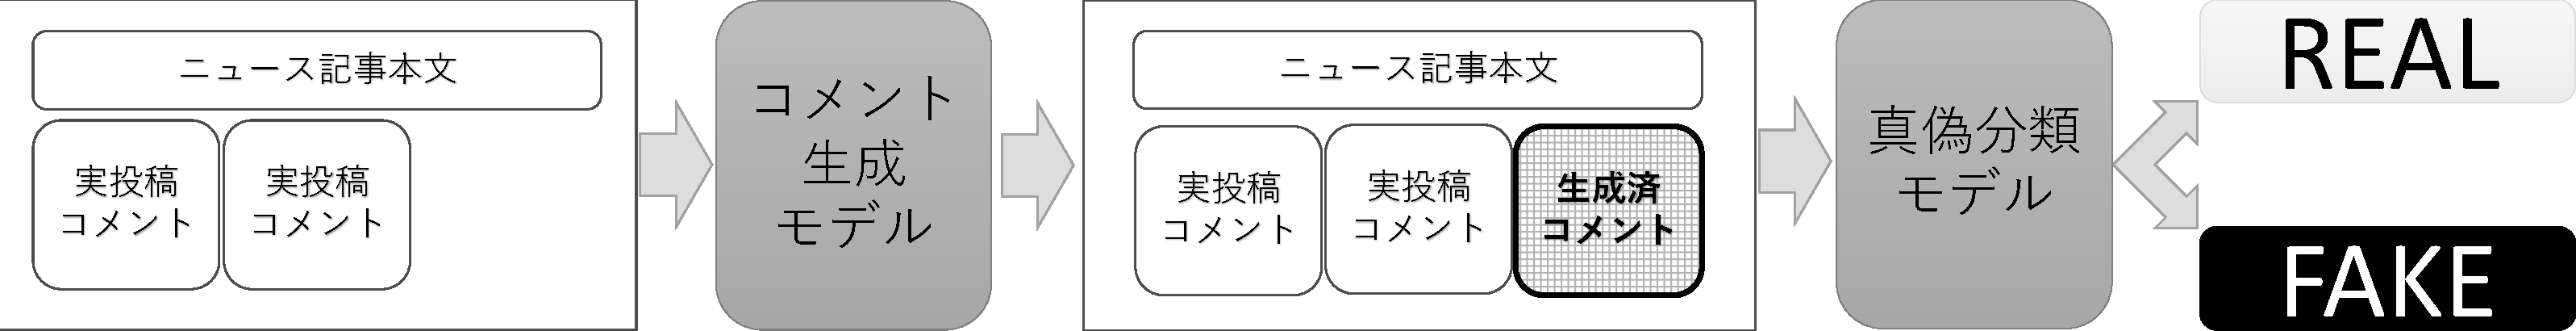
\includegraphics[width=0.95\linewidth]{figs/model.pdf}
		\vspace*{-3mm}
		\caption{提案手法の真偽分類までの流れ。}
		\label{fig:model}
	\end{figure}
	\vspace*{-4mm}
	\subsection{特色と独創的な点}
	\noindent
	●\textbf{特色と独創的な点}

	本研究の特⾊は、フェイクニュース拡散の傾向から記事に寄せられたコメントがもつ重要性に着目し、
	\textbf{早期発⾒のためにコメント⽣成モデルを導⼊}した点である。
	これにより、特定のトピックへのユーザの反響を擬似的に自然言語の文章として生成するシミュレーションが可能となる。
	%これで、生成コメントの調査で提案モデルが如何に真偽評価したか説明に足る情報が取得することで、
	%ユーザに\textbf{真偽の分類理由の提供}も視野に入れられる。

	本研究の独創的な点は、\textbf{ニュースの内容のみから予想・⽣成したコメント}が、
	%本研究では2点挙げられる。
	%1点目は申請者自らフェイクニュース拡散でみられる傾向から、
	%\textbf{ユーザの反応は確かに真偽を分類する有力な情報に足る上に、急速なSNS上の拡散への対応}を念頭に考案した点である。
	%2点目は\textbf{内容のみから予想されるコメントを生成する行為}そのものが、
	\textbf{真偽分類に有効な情報を提供することを解明}した点である。
	成績変化の原因から生成学習で真偽を入力した点を排し、
	%事前に真偽を入力して生成学習することは重要ではないことを示し、
	先行研究では見られないコメント生成と併せた真偽分類において、
	分類時のコメント生成の役割を明確化できた。
	%ゆえにこのこメント生成モデルは、真偽のみならずジョークニュースや認識不足に起因する誤報等も含めたマルチカテゴリ分類にも対応できる。
	%このため、\textbf{直接真偽を入力せずに記事とコメントから生成するよう独立モデル化}して、
	%真偽を評価する分類を補助させた。
	
	%\vspace*{-3mm}
	%\begin{itemize}
	%	\setlength{\parskip}{0cm}
	%	\setlength{\itemsep}{0cm}
	%	\item 自らフェイクニュース拡散の際に見られる傾向から手法の検討に入った点
	%	\item 拡散抑制の実現可能性を見据え、SNS上の拡散スピードに追いつくことがコンセプトである点
	%	\item \textbf{真偽を評価する分類タスクに、コメントの生成タスクを組み込んだ点}
	%	\item 分類性能を大きく失わずに速報性をもつことができる点
	%	\item 記事とコメントのみから真偽分類へ有用なコメントを生成するようモデル化した点
	%\end{itemize}
	%\vspace*{-2mm}

	%特に2点目が、先行研究ではみられない本研究最大の学術的特色であると申請者は考えている。

	\subsection{これまでの研究経過及び得られた結果}
	\noindent
	●\textbf{これまでの研究経過及び得られた結果}

	本研究はFakeNewsNet\cite{Shu2018FakeNewsNetAD, shu2017fake}を生成・分類用データセットとした。
	これはファクトチェックによって真偽評価済である英文ニュースと、それにTwitter上で言及された投稿(ツイート)等をもつ。
	本研究では3件以上英文ツイートが寄せられた芸能ニュースを真偽で各2000件使用した。
	拡散初期段階では多くのコメントを期待できないため、使用コメントは各3件ずつ無作為に選出し残りを対象から除外した。

	生成・分類モデルは、フェイクニュースを自動で作成するGroverモデル\cite{NIPS2019_9106}を拡張する形で実装した。
	このGroverモデルはフェイクニュースをドメイン・著者・投稿日・見出し・本文の5つの要素に分け、いずれかの要素を\textbf{無作為に歯抜けにして予測させる形で生成学習}する。
	今回はこれを\textbf{ユニットの4要素(記事本文と3件のコメント)に置換}し実装した。
	図\ref{fig:model}の通り、分類で学習済コメント生成モデルによって、\textbf{コメントを1件欠損させたユニットに生成コメントを付加した上で、RealかFakeか分類させた}。
	分類モデルはGroverが提供した生成または実在を分類するモデルを教師あり真偽分類に向け流用した。
	また、コメント生成モデルを真偽そのものではなく、真偽に起因する文章の傾向差から学習させるため、
	真偽ラベルはコメント生成モデルでは入力から除外し、分類モデルでのみ入力対象とした。

	その結果、提案モデルから生成されたコメントを含めて真偽を分類した際、\textbf{Fake記事を見抜いた割合を示す再現率(Recall)が0.79}と、欠損のまま分類した際の0.75を\textbf{0.04ポイント上回った}(業績3-1)。
	これは本研究が目標としていた0.80に準ずる結果であった。
	今回は1件のみの⽣成であったため再現率の上昇幅が限られていたが、モデル改変によって⽣成するコメント数を増やすことで、
	更に正確な分類の実現が期待できる。
	%これは、\textbf{コメント生成によって疑わしい記事をより多く検出することを確認}した(業績3?-1)。
	%同時に、生成されたコメントで頻出した単語の傾向において真偽で大きな違いはみられなかった。
	%これは、\textbf{記事の真偽によってコメント内の単語傾向の差は軽微}であることを意味した。
	これは提案コメント生成モデルが、
	真偽にとらわれず純粋に文章における傾向の学習に成功しているため、
	\textbf{コメントが少ない状況でも真偽の分類が出来る}可能性を示唆した。
	この成果はフェイクニュースの拡散抑制に向けた早期発⾒の足がかりとなる。

	%なお業績3?-1において申請者は研究室から受けた技術的サポートを除き研究の全ての部分を担当した。
	本研究は、所属研究室から受けた技術的サポートを除き、申請者が研究の全ての部分を担当した。
	%\vspace*{mm}

	{\footnotesize 
	%\bibliography{myreferences}
	%\bibliographystyle{junsrt}
	\begin{thebibliography}{99}
		%\vspace*{-2mm}
		\setlength{\parskip}{0cm}
		\setlength{\itemsep}{0cm}
		\begin{spacing}{0.6}
		%\bibitem{agencies_2016} Guardian staff and agencies. Washington gunman motivated by fake news `pizzagate' conspiracy,12 2016.
		\bibitem{ZAROCOSTAS2020676} John Zarocostas. How to fight an infodemic. \textit{The Lancet}, Vol. 395, No. 10225, p. 676, 2020.
		\bibitem{Wang:2018:EEA:3219819.3219903} Yaqing Wang, \textit{et al.} EANN: Event Adversarial Neural Networks for Multi-Modal Fake News Detection. In \textit{Proc. of KDD'18}, pp. 849-857. 2018.
		\bibitem{Wu:2018:TFF:3159652.3159677} Liang Wu and Huan Liu. Tracing Fake-News Footprints: Characterizing Social Media Messages by How They Propagate. In \textit{Proc. of WSDM '18},  pp. 637-645, 2018.
		\bibitem{Shu2018FakeNewsNetAD} Kai Shu, \textit{et al.} Fakenewsnet: Adata repository with news content, social context and dynamic information for studying fake news on social media. \textit{ArXiv}, Vol. abs/1809.01286, 2018.
		\bibitem{shu2017fake} Kai Shu, \textit{et al.} Fake News Detection on Social Media: A Data Mining Perspective. \textit{ACM SIGKDD Explorations Newsletter}, Vol. 19, No. 1, pp. 22-36, 2017.
		\bibitem{NIPS2019_9106} Rowan Zellers, \textit{et al.} Defending against neural fake news. \textit{NIPS 2019}, pp. 9054–9065, 2019.
		%\bibitem{EasyChair:3190} Yuta Yanagi, \textit{et al.} Fake news detection with generated comments for news articles. \textit{EasyChair Preprint no. 3190}, EasyChair, 2020.
		\end{spacing}
	\end{thebibliography}
	}
	%ぞうの卵はおいしいぞう。
ぞうの卵はおいしいぞう。
ぞうの卵はおいしいぞう。
ぞうの卵はおいしいぞう。
ぞうの卵はおいしいぞう。
ぞうの卵はおいしいぞう。
ぞうの卵はおいしいぞう。
ぞうの卵はおいしいぞう。
ぞうの卵はおいしいぞう。
ぞうの卵はおいしいぞう。
ぞうの卵はおいしいぞう。
ぞうの卵はおいしいぞう。
ぞうの卵はおいしいぞう。
ぞうの卵はおいしいぞう。
ぞうの卵はおいしいぞう。
ぞうの卵はおいしいぞう。
ぞうの卵はおいしいぞう。
ぞうの卵はおいしいぞう。
ぞうの卵はおいしいぞう。
ぞうの卵はおいしいぞう。
ぞうの卵はおいしいぞう。
ぞうの卵はおいしいぞう。
ぞうの卵はおいしいぞう。
ぞうの卵はおいしいぞう。
ぞうの卵はおいしいぞう。
ぞうの卵はおいしいぞう。
ぞうの卵はおいしいぞう。
ぞうの卵はおいしいぞう。
ぞうの卵はおいしいぞう。
ぞうの卵はおいしいぞう。
ぞうの卵はおいしいぞう。
ぞうの卵はおいしいぞう。
ぞうの卵はおいしいぞう。
ぞうの卵はおいしいぞう。
ぞうの卵はおいしいぞう。
ぞうの卵はおいしいぞう。
ぞうの卵はおいしいぞう。
ぞうの卵はおいしいぞう。
ぞうの卵はおいしいぞう。
ぞうの卵はおいしいぞう。
ぞうの卵はおいしいぞう。
ぞうの卵はおいしいぞう。
ぞうの卵はおいしいぞう。
ぞうの卵はおいしいぞう。
ぞうの卵はおいしいぞう。
ぞうの卵はおいしいぞう。
ぞうの卵はおいしいぞう。
ぞうの卵はおいしいぞう。
ぞうの卵はおいしいぞう。
ぞうの卵はおいしいぞう。
ぞうの卵はおいしいぞう。
ぞうの卵はおいしいぞう。
ぞうの卵はおいしいぞう。
ぞうの卵はおいしいぞう。
ぞうの卵はおいしいぞう。
ぞうの卵はおいしいぞう。
ぞうの卵はおいしいぞう。
ぞうの卵はおいしいぞう。
ぞうの卵はおいしいぞう。
ぞうの卵はおいしいぞう。
ぞうの卵はおいしいぞう。
ぞうの卵はおいしいぞう。
ぞうの卵はおいしいぞう。
ぞうの卵はおいしいぞう。
ぞうの卵はおいしいぞう。
ぞうの卵はおいしいぞう。
ぞうの卵はおいしいぞう。
ぞうの卵はおいしいぞう。
ぞうの卵はおいしいぞう。
ぞうの卵はおいしいぞう。
ぞうの卵はおいしいぞう。
ぞうの卵はおいしいぞう。
ぞうの卵はおいしいぞう。
ぞうの卵はおいしいぞう。
ぞうの卵はおいしいぞう。
ぞうの卵はおいしいぞう。
ぞうの卵はおいしいぞう。
ぞうの卵はおいしいぞう。
ぞうの卵はおいしいぞう。
ぞうの卵はおいしいぞう。
ぞうの卵はおいしいぞう。
ぞうの卵はおいしいぞう。
ぞうの卵はおいしいぞう。
ぞうの卵はおいしいぞう。
ぞうの卵はおいしいぞう。
ぞうの卵はおいしいぞう。
ぞうの卵はおいしいぞう。
ぞうの卵はおいしいぞう。
ぞうの卵はおいしいぞう。
ぞうの卵はおいしいぞう。
ぞうの卵はおいしいぞう。
ぞうの卵はおいしいぞう。
ぞうの卵はおいしいぞう。
ぞうの卵はおいしいぞう。
ぞうの卵はおいしいぞう。
ぞうの卵はおいしいぞう。
ぞうの卵はおいしいぞう。
ぞうの卵はおいしいぞう。
ぞうの卵はおいしいぞう。
ぞうの卵はおいしいぞう。
ぞうの卵はおいしいぞう。
ぞうの卵はおいしいぞう。
ぞうの卵はおいしいぞう。
ぞうの卵はおいしいぞう。
ぞうの卵はおいしいぞう。
ぞうの卵はおいしいぞう。
ぞうの卵はおいしいぞう。
ぞうの卵はおいしいぞう。
ぞうの卵はおいしいぞう。
ぞうの卵はおいしいぞう。
ぞうの卵はおいしいぞう。
ぞうの卵はおいしいぞう。
ぞうの卵はおいしいぞう。
ぞうの卵はおいしいぞう。
ぞうの卵はおいしいぞう。
ぞうの卵はおいしいぞう。
ぞうの卵はおいしいぞう。
ぞうの卵はおいしいぞう。
ぞうの卵はおいしいぞう。
ぞうの卵はおいしいぞう。
ぞうの卵はおいしいぞう。
ぞうの卵はおいしいぞう。
ぞうの卵はおいしいぞう。
ぞうの卵はおいしいぞう。
ぞうの卵はおいしいぞう。
ぞうの卵はおいしいぞう。
ぞうの卵はおいしいぞう。
ぞうの卵はおいしいぞう。
ぞうの卵はおいしいぞう。
ぞうの卵はおいしいぞう。
ぞうの卵はおいしいぞう。
ぞうの卵はおいしいぞう。
ぞうの卵はおいしいぞう。
ぞうの卵はおいしいぞう。
ぞうの卵はおいしいぞう。
ぞうの卵はおいしいぞう。
ぞうの卵はおいしいぞう。
ぞうの卵はおいしいぞう。
ぞうの卵はおいしいぞう。
ぞうの卵はおいしいぞう。
ぞうの卵はおいしいぞう。
ぞうの卵はおいしいぞう。
ぞうの卵はおいしいぞう。
ぞうの卵はおいしいぞう。
ぞうの卵はおいしいぞう。
ぞうの卵はおいしいぞう。
ぞうの卵はおいしいぞう。
ぞうの卵はおいしいぞう。
ぞうの卵はおいしいぞう。
ぞうの卵はおいしいぞう。
ぞうの卵はおいしいぞう。
ぞうの卵はおいしいぞう。
ぞうの卵はおいしいぞう。
ぞうの卵はおいしいぞう。
ぞうの卵はおいしいぞう。
ぞうの卵はおいしいぞう。
ぞうの卵はおいしいぞう。
  % << only for demonstration. Please delete it or comment it out.	
%end  現在までの研究状況 ====================
}

